\documentclass{article}
\usepackage{tikz, comment}
\usepackage{pifont}
\usepackage{fontspec}
\usetikzlibrary{arrows, decorations.markings, decorations.pathreplacing}
\begin{comment}
:Title: Not defined yet
:Tags: function;form;focus;directrix;curve;conic
:Author: Prof.Hu Ji-shan, HKUST
:Slug: No name yet

Description Here.........
\end{comment}
\begin{document}\centering

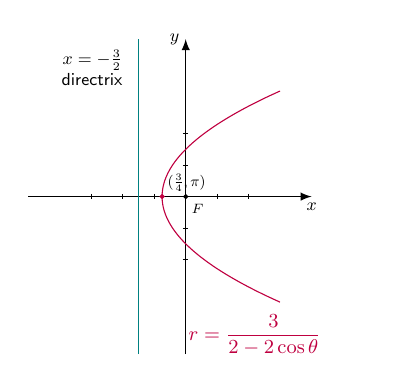
\begin{tikzpicture}[>=latex,xscale=.5/1.25, yscale=.5/1.25][font=\sf\small]

%\draw[xstep=1cm,ystep=1cm,color=gray!80] (0, -1) grid (8, 8);

\draw[->] (-5, 0) -- (4, 0)node[below, scale=0.7] {$x$};
\draw[->] (0, -5) -- (0, 5)node[left, scale=0.7] {$y$};

\draw[teal, samples=100, smooth, domain=-5:5, variable=\y]
plot ({-3/2}, {\y});

\node[left, xshift=0, yshift=0, scale=0.7] at ({-3/2}, 4) {$\begin{array}{r}x=-\frac{3}{2}\\\hbox{directrix}\end{array}$};

\node[purple, xshift=25, yshift=-50, scale=0.8] at (0,0) {$\displaystyle r = \frac{3}{2-2\cos \theta}$};

\draw[fill, xscale= 1.25, yscale= 1.25] ({0/1}, {0/1}) circle(0.05);

\draw[purple, fill, xscale= 1.25, yscale= 1.25] ({-(3/4)/1.25}, {0/1.25}) circle(0.05)node[black, right, xshift=0, yshift=5, scale=0.6] {$(\frac{3}{4},\pi)$};

\foreach \x in {-3,-2,-1,1,2}
\draw (\x,2pt*1.25) -- (\x,-2pt*1.25)
node[anchor=north] {}%{\tiny$\x$}
;
\foreach \x in {}
\draw (\x,2pt*1.25) -- (\x,-2pt*1.25)
node[anchor=south] {\tiny$\x$}
;
\foreach \y in {-2,-1, 1,2}
\draw (-2pt*1.25,\y) -- (2pt*1.25,\y)
node[anchor=east] {}%{\tiny $\y$}
;

\node[scale=0.7] at ({0.2*1.5*1.25}, {-0.2*1.5*1.25}) {\scriptsize$F$};

\clip[] (-3, -4.5) rectangle (6, 4.5);
\draw[purple, samples=100, smooth, domain=pi-2.3:pi+2.3, variable=\t]
plot ({3/(2-2*cos(\t r))*cos(\t r)}, {3/(2-2*cos(\t r))*sin(\t r)});

\end{tikzpicture}
\end{document}